\documentclass[11pt, notitlepage,abstracton,oneside]{article}   	% use "amsart" instead of "article" for AMSLaTeX format
\usepackage{geometry}                		% See geometry.pdf to learn the layout options. There are lots.
\geometry{letterpaper}                   		% ... or a4paper or a5paper or ... 
\usepackage{graphicx}				% Use pdf, png, jpg, or eps§ with pdflatex; use eps in DVI mode
								% TeX will automatically convert eps --> pdf in pdflatex		
\usepackage{amssymb}

\title{Analysis of Medical Device Failure Reports from the MAUDE Database: A Data Mining Approach}
\author{Simon Diemert, Scott Low, Paul Moon}
\date{March 23rd 2015}							% Activate to display a given date or no date

\begin{document}
\maketitle

\begin{abstract}

%REFERENCE FORMAT: http://cs.stanford.edu/people/widom/paper-writing.html#related

\thispagestyle{empty}
Lorem Ipsum is simply dummy text of the printing and typesetting industry. Lorem Ipsum has been the industry's standard dummy text ever since the 1500s, when an unknown printer took a galley of type and scrambled it to make a type specimen book. It has survived not only five centuries, but also the leap into electronic typesetting, remaining essentially unchanged. It was popularised in the 1960s with the release of Letraset sheets containing Lorem Ipsum passages, and more recently with desktop publishing software like Aldus PageMaker including versions of Lorem Ipsum.
\end{abstract}

\tableofcontents

\clearpage
\newpage
\setcounter{page}{1}
\section{Introduction}
Modern medicine relies heavily on technology to support the delivery of treatments and care. These technologies are described by the umbrella term ``medical devices" which encompasses any combination of mechanical, electrical, software devices that are used in medical care. The implications of these devices failing can range from minor annoyances to death. Adverse events related to medical devices in the United States are reported to the Food and Drug Administration (FDA). These reports are stored in the \textbf{Ma}nufacturer and \textbf{U}ser Facility \textbf{D}evice \textbf{E}xperience (MAUDE) database and are publicly accessible. The MAUDE database contains approximately 3.7 million records dating back to 1991. 

Previous works have focused on analyzing the data in the MAUDE database to extract trends related to specific devices \cite{weber_preliminary_2011}. However, many of these analyses have been conducted using a manual review process that does not lend itself well to analyzing the large number of records available in the MAUDE database. The FDA has recently made the data accessible via its openFDA API which allows programmatic access to the data. To the best of our knowledge, no work analyzing data obtained from this new API has been published.

Health care is a complex domain that requires medical devices to interact with humans in increasingly complicated ways. There are many examples of adverse medical events that were caused by a combination of a device and human users. Horsky conducted an analysis of such an event \cite{horsky_2005}. Safety analyses of medical devices must consider more than just the device. They must also consider how the device interacts with human actors \cite{karsh_health_2010}. Leveson has presented general a model for analyzing the behaviour of complex sociotechnical systems called the STAMP model. The STAMP model describes a system as a feedback control loop with a controlled process being actuated and sensed by a human actor \cite{leveson_engineering_2012}. Work by Mason-Blakely and Weber has tailored this model for analysis of software in health care. This model is shown in Figure \ref{fig:stamp-emr} below \cite{stamp_emr_2011}.

\begin{figure}[ht]
	\centering
	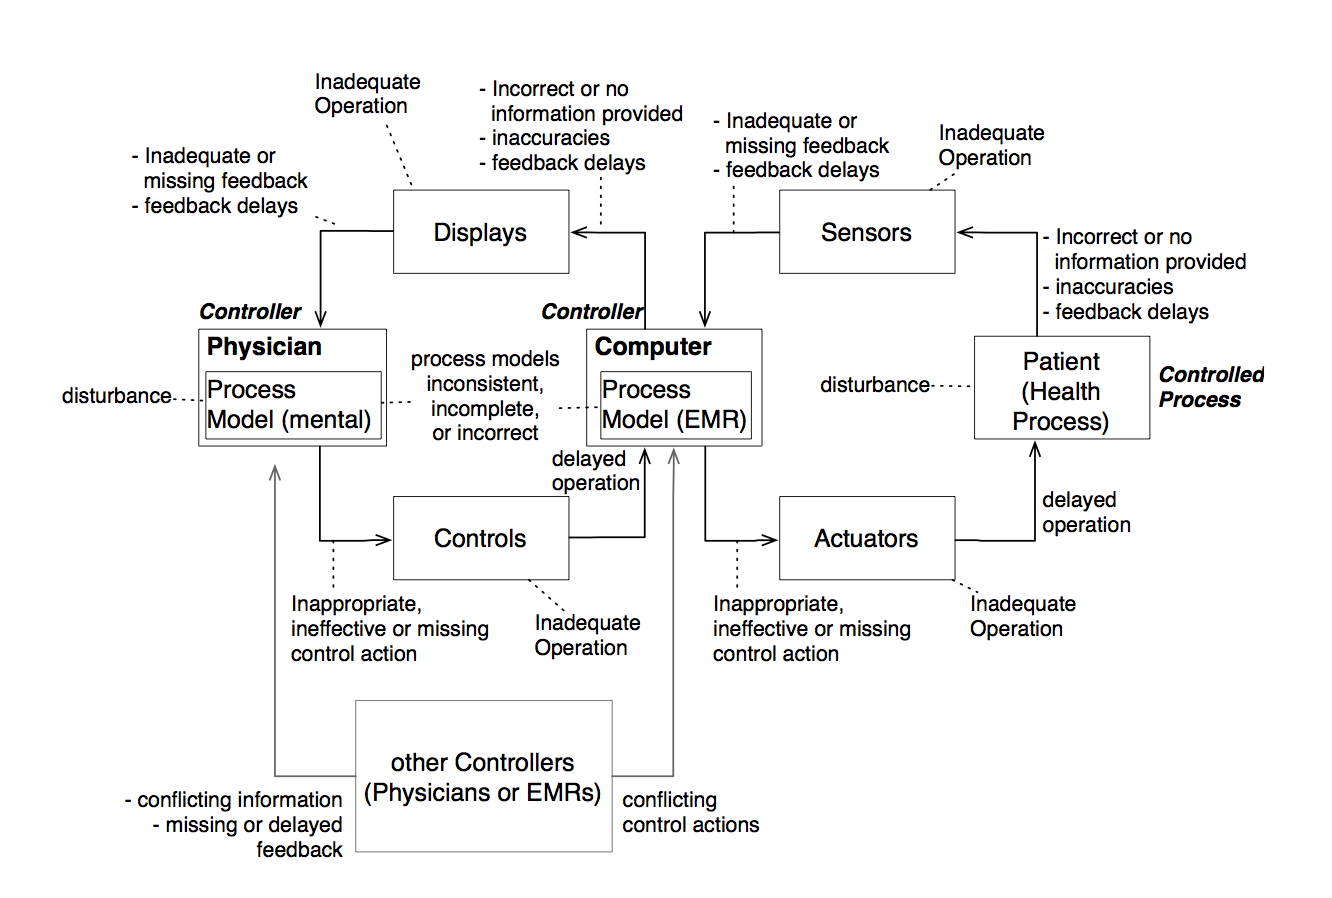
\includegraphics[width=0.95\textwidth]{figures/stamp-emr}
	\caption{STAMP - EMR model from \cite{stamp_emr_2011}}
	]\label{fig:stamp-emr}
\end{figure}

Mason-Blakey and Habibi used the STAMP EMR model to classify 350 adverse event reports related to software in the MAUDE database (not yet published). This classification was conducted by manually inspecting the natural language summary of each event. A number of different classes (related to the STAMP EMR model) were assigned to each record depending on the reviewer's understanding on the adverse event and how it fits into the STAMP EHR model. The categories used were: 

\begin{itemize}
	\item Care Provider
	\item Point of Care Sensor
	\item Point of Decision Display
	\item Point of Care Actuator
	\item Point of Decision Control
	\item Medical Device Decision Support (MDDS)
	\item Technical Process
\end{itemize}

In this project the MAUDE database was examined algorithmically using standard data mining techniques. Two different approaches were used to analyze data from MAUDE database:  i) analysis of the metadata for each record to predict the outcome of the event (injury, death, etc.); ii) analysis of the natural language description of the adverse event in an attempt to classify the outcome of each record (as outlined in the STAMP EMR model). The remainder of this paper is structured as follows: section 2 describes the methods used to collect and analyze this data; section 3 presents results; and section 4 provides a discussion of results and outlines strengths and weaknesses of the aforementioned approaches. 

\section{Methods}
This section describes two approaches to analyzing the data from the MAUDE. The first approach used the metadata from a large number of events to attempt to predict event outcomes. The second approach used a small set of events (previously classified by Mason-Blakey and Habibi) and attempted to classify these based on the natural language summary of the adverse event. 

\subsection{Approach I: Metadata Analysis}
The first approach that was considered for classifying records obtained from the MAUDE was the analysis of important metadata fields. In order to complete this approach, a Python script was written to mine the openFDA API over a specified date range and obtain raw JSON dumps of the data. Once this was complete, the results were manually inspected and a list of important metadata attributes was created. These attributes were as follows:

\begin{itemize}
	\item \textbf{device\_operator:} The person using the medical device at the time of the adverse event.
	\item \textbf{manufacturer\_name:} The name of the manufacturer who created the device in question.
	\item \textbf{reporter\_occpation\_code:} The occupation code of the person who reported the failure of the device in question.
	\item \textbf{device\_report\_product\_code:} Three-letter FDA Product Classification Code. Medical devices are classified under 21 CFR Parts 862-892.
	\item \textbf{expired:} A boolean flag with a value of \textit{true} if the device was past its manufacturer-provided expiry date at the time its failure was reported.
\end{itemize}

Once this list of metadata attributes was obtained, a second Python script was created to merge and sanitize the collected data, filtering out metadata attributes that were deemed unimportant before creating a .arff file for data analysis in Weka.

\subsubsection{Data Collection}
As previously described, the first step of the metadata analysis approach was to write a Python script that was able to scrape the openFDA API for all records within a specified date range. After obtaining an API key from openFDA, the script was written such that it grabbed records starting from January 1, 2014 in 100-record chunks as this is the maximum number of records that was allowed to be returned in a single API call. 

It is worth noting that for the sake of virtual memory management, the script would write 10,000 records to a single text file before closing that file and opening a new one for the next 10,000 records. This also helped to ensure that as much data as possible would be preserved in the event of a script failure (due to, for example, loss of internet connection during execution). 

Once the script was written and run for the first time, it was noted that a large number of HTTP 403 errors were being returned from the openFDA API. After consulting the API documentation, it was determined that this was due to the script exceeding the maximum number of API requests allowed per second. As a result, a timeout of half a second had to be added to each outgoing request to ensure that the number of requests per second remained below this limit.

For the scope of this experiment, the first 50,000 of the 602,117 medical device failure records from the year 2014 were used in this approach. It is important to note, however, that the previously described script, is able to download any number of records between any range of dates. In the future, it would be interesting to run the script for longer to observe the effects that a larger dataset has on the results of the classification process.

\subsubsection{Data Pre-Processing}
The data pre-processing phase of the first approach was by far the most time consuming phase due to a number of challenges that were experienced when attempting to merge and parse the 10,000-record JSON dumps that were obtained in the data collection step into a single .arff file. To process the data, a second Python script was run that would open each of the 10,000-record JSON dumps, extract the important metadata attributes (as described in section 2.1), and write these to a .arff file. Non-unicode characters in the JSON dumps, however, meant that any records containing such characters could not be written to the .arff and needed to be skipped. As a result, ASCII encoding of each metadata attribute for each record needed to be attempted before writing it to the .arff if and only if all encoding attempts for the specified record succeeded.

Once the .arff was created and loaded into Weka, it became apparent that due to the nominal nature of the metadata attributes, all possible values for each of the metadata attributes needed to be included in each one's respective @ATTRIBUTE definition at the beginning of the .arff. As a result, code to extract all possible values for each metadata attribute (while removing duplicates and skipping records with null values)	 needed to be written. 

Upon rerunning the script with the aforementioned logic in place, a .arff file with fully defined, nominal attributes was created and could be loaded into Weka for analysis. 

\subsubsection{Data Analysis}
The data analysis phase for this approach was relatively straightforward. The .arff generated in the previous step was loaded into Weka and a Naive Bayes classifier with 10 fold cross-validation was used to analyze the data. After running the classifier, it was observed that 76.67\% of all records were classified correctly.

It is worth mentioning that a number of other classifiers, such as J48, Bayesian Network, and ID3 were also run simply to observe results, but due to the large amount of data being processed, none of these produced meaningful results. 

\subsection{Approach II: Record Categorization}
\subsubsection{Data Collection}

\subsubsection{Data Pre-Processing}

\subsubsection{Data Analysis}

\section{Results}

\subsection{Approach I: Metadata Analysis}

\subsection{Approach II: Record Categorization}

\section{Discussion}
Lorem Ipsum is simply dummy text of the printing and typesetting industry. Lorem Ipsum has been the industry's standard dummy text ever since the 1500s, when an unknown printer took a galley of type and scrambled it to make a type specimen book. It has survived not only five centuries, but also the leap into electronic typesetting, remaining essentially unchanged. It was popularised in the 1960s with the release of Letraset sheets containing Lorem Ipsum passages, and more recently with desktop publishing software like Aldus PageMaker including versions of Lorem Ipsum.

\section{Conclusion}
Lorem Ipsum is simply dummy text of the printing and typesetting industry. Lorem Ipsum has been the industry's standard dummy text ever since the 1500s, when an unknown printer took a galley of type and scrambled it to make a type specimen book. It has survived not only five centuries, but also the leap into electronic typesetting, remaining essentially unchanged. It was popularised in the 1960s with the release of Letraset sheets containing Lorem Ipsum passages, and more recently with desktop publishing software like Aldus PageMaker including versions of Lorem Ipsum.


\bibliographystyle{plain}
\bibliography{report}


\end{document}  
